\documentclass[acmtog, authorversion]{acmart}

\usepackage{booktabs} % For formal tables

% TOG prefers author-name bib system with square brackets
\citestyle{acmauthoryear}
\setcitestyle{square}


\usepackage[ruled]{algorithm2e} % For algorithms
\renewcommand{\algorithmcfname}{ALGORITHM}
\SetAlFnt{\small}
\SetAlCapFnt{\small}
\SetAlCapNameFnt{\small}
\SetAlCapHSkip{0pt}
\IncMargin{-\parindent}

% Metadata Information




\acmYear{2017}
\acmMonth{5}

% Copyright
%\setcopyright{acmcopyright}
%\setcopyright{acmlicensed}
\setcopyright{rightsretained}
%\setcopyright{usgov}

%\setcopyright{cagov}
%\setcopyright{cagovmixed}

% DOI

% Paper history
\received{Mai 2017}


% Document starts
\begin{document}
% Title portion
\title{Video Style Transfer for Videos} 
\author{Simon Sternsdorf}

\affiliation{%
  \institution{Technical University Munich}
}

\renewcommand\shortauthors{Sternsdorf}

\begin{abstract}
In art, redrawing an image with a certain artistic style is often useful. Doing it by hand is however very elaborate and can be very time consuming. 
We will present a method to transfer the style of an image to another with help of a neural network in a fraction of the time needed to do this by hand. We will also talk about a method to transfer the style of an image to a whole video sequence. Stable video generation is possible with help of new loss functions. Also methods to counteract against strong motion or occlusion are included. 
\end{abstract}




%
% The code below should be generated by the tool at
%
% Please copy and paste the code instead of the example below. 
%

%
% End generated code
%


\keywords{Video Style transfer, video recognition, Convolutional Neural Network}





\maketitle


\section{Introduction}
In Summer 2016, a smartphone app called Prisma had its 15 minutes of fame as it hit 10 million downloads in the Google Play Store very quickly. \cite{Prisma}
In the app you can upload a picture from your smartphone and afterwards choose from a collection of art pieces. The style of the art piece gets applied to your picture. 
The whole process only takes up to 10 seconds. To achieve this speed the service behind the app uses a neural network. \cite{Paper1} We will try to explain how the neural network works and also how we can apply this concept to whole video sequences. 

\section{Picture recognition}
First we will talk about the concepts of the neural network to recognize the content and the style of a picture. We use convolutional neural networks for this task. CNNs are a class of Deep neural networks and are very potent in image processing. \cite{Paper1} Convolutional Neural Networks have different layers which they use to process an image in different steps. We will showcase these with help of figure \ref{fig:Convolution}. 
\begin{figure*}
\centering
	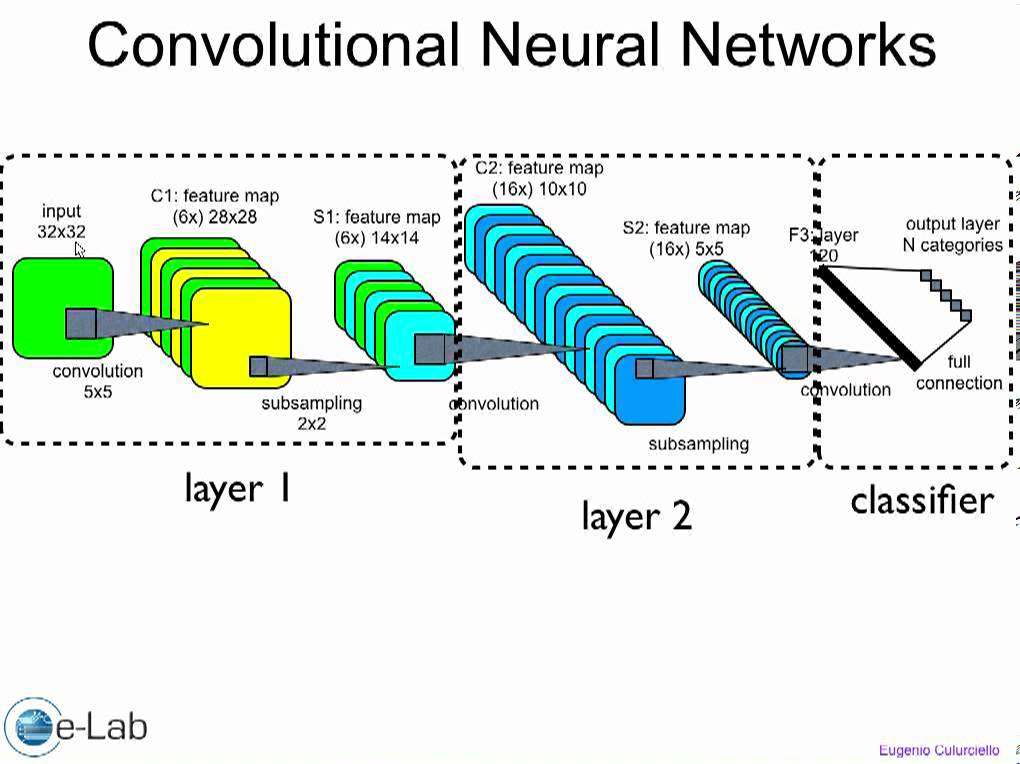
\includegraphics[width=0.5\textwidth]{figures/convolution.jpg}
	\caption{Work of a CNN \citep{convo}}
	\label{fig:Convolution}
\end{figure*} 

Here we see the basic principle of the work of a CNN. First we have a convolution phase, where we apply convolution to all the pixels of our image. This reduces the size of our image, since we "lose" the pixels at the borders of our picture. As a result we get feature maps as an output. Afterwards we subsample the feature maps, reducing their size by the factor 2. These feature maps are the input for the next layer of our CNN. As you can see, each layer acts for us as a feature identifier. \cite{convo} The first layers check for very simple and small characteristics like edges or parts of curves. Layers towards the end of our CNN get feature maps which have been sub sampled multiple times. They consequently identify higher level features of our image. In the end of the CNN we have a fully connected layer. This layer takes the output of our last subsampling as an input and gives us an n-dimensional vector as an output. We get probabilities for our n classes the CNN had to choose from. \citep{convo} We are not interested in the object the convolutional neural network has identified in our pictures. When CNNs are trained to identify certain objects, they develop a representaion of the image they are working on in the different layers. These representations depict the object information in a lot more precise way. \citep{Paper1} Since our goal is to extract the content of a picture and we do not care about specific pixel values, we want to get the representations of the different layers of the CNN. This is possible, since we can reconstruct the image of a layer from the feature map. This can be seen very clearly in figure \ref{fig:NetworkModel}. 
\begin{figure*}
	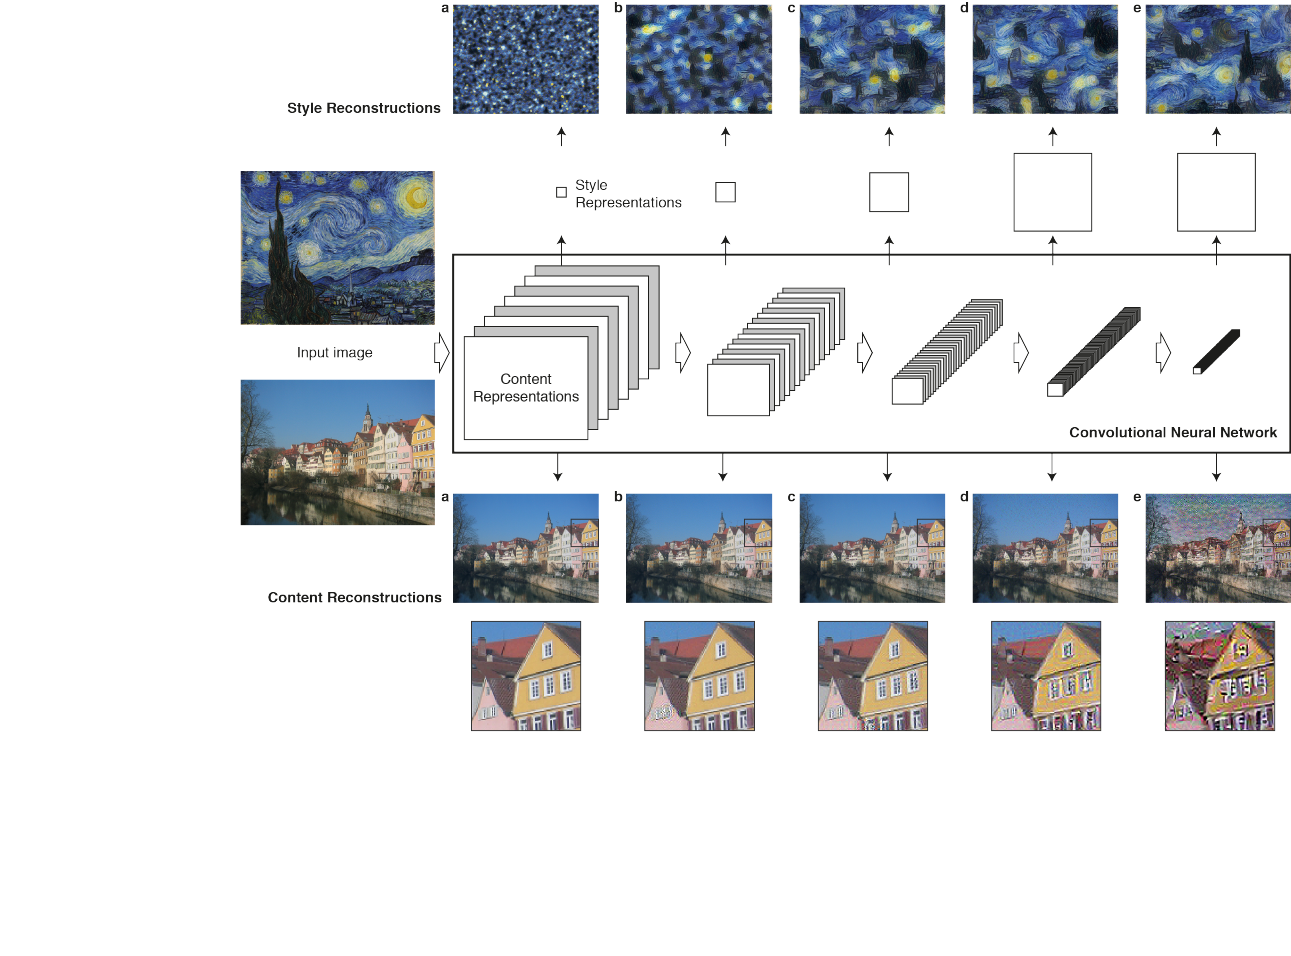
\includegraphics[width=1\textwidth]{figures/network_model.png}
	\caption{Reconstruction of content and style \citep{Paper1}}
	\label{fig:NetworkModel}
\end{figure*}

Here we have the content and the style reconstruction. Seemingly the representation in the higher layers of the CNN contains the content of the image, the exact values of every pixel are however lost. In lower levels the picture pretty much looks like the original we used, the exact pixel value gets preserved. Since we only want the content, we use the feature response from higher levels. $\newline$
For the style we use a special texture CNN. The CNN is used to identify different textures in pictures and thus we can get texture information out of the CNN. For that we combine the feature correlations of multiple layers of the CNN. \citep{Paper1} This gives us a good representation of the texture of an image, with no direct representation of the content. The representations acquire the general appearance with the local colors and localized structures. $\newline$
These results imply: 
\begin{itemize}
\item Content and style of an image are separable
\item Both representations can be changed independently
\item Mixing of content and style of two different source images is possible
\end{itemize}

\subsection{Method of content reconstruction}
For the content reconstruction we need to visualize the representation of the image on a layer. To achieve this we perform gradient descent on a white noise image.
Our goal is to find the white noise image to match the feature response of our original image in the higher levels of the CNN. $\newline$
Notation: $\overrightarrow{p}$ is our original image, $\overrightarrow{x}$ our white noise image. $P^l$ and $F^l$ are their respective feature responses in layer $l$. $\newline$ We now need the squared error loss between the feature representations of $\overrightarrow{p}$ and $\overrightarrow{x}$. For that we define the loss function: 
$$ \mathcal{L}_{content}(\overrightarrow{p},\overrightarrow{x},l) = \frac{1}{2}\sum_{i,j}(F_{ij}^l - P_{ij}^l)^2$$ 
To compute the gradient we need the derivative of the loss considering if the layer l has activations: 
$$ \frac{\partial \mathcal{L}_{content} }{\partial F_{ij}^l} = \begin{cases}
     															(F^l - P^l)_{ij} \quad \text{if} \quad F_{ij}^l > 0 \\
     															0 \qquad \quad \qquad \text{if} \quad F_{ij}^l < 0
   																\end{cases} $$
From here we can use back-propagation to compute the gradient. The idea is to choose a different $\overrightarrow{x}$ until we get a similar feature response in a high layer of our CNN as we got with our original image $\overrightarrow{p}$. 
\subsection{Method of style reconstruction}
To reconstruct the style of an image we first create a style representation on top of our CNN. We calculate the feature responses in the different layers and represent the correlations between them in a Gram matrix $G^l \in \mathbb{R}^{N_l \times N_l} $. Here $G_{ij}^l$ is the inner product between the vectorized feature map $i$ and $j$ in layer $l$. As a formula: $$G_{ij}^l = \sum _k F^l_{ik} F^l_{jk} $$ With this we can reconstruct the style of an image very similarly to how we reconstructed the content of an image. We perform gradient descent on an white noise image. For that we minimize the mean squared distance between the entries of the Gram matrices of the original image and of the white-noise image. As a formula: $\newline \newline$
When we have $\overrightarrow{a}$ as our artwork and $\overrightarrow{x}$ as the image that is generated, as well as $A^l$ and $ G^l$ as the respective style representations in layer $l$ : $$E_l = \frac{1}{4N_l^2M_l^2}\sum_{ij}(G^l_{ij} - A^l_{ij})^2$$ 
This is the loss in one layer. As our total style loss function we get: $$\mathcal{L}_{style}(\overrightarrow{a},\overrightarrow{x}) = \sum^L_{l=0}w_lE_l$$
Here $w_l$ is a weighting factor. $\newline$
\subsection{Total Loss function}
We now want to combine the content of one image with the style of an artwork. To achieve that we minimize the distance of a white-noise image from the content representation of our image in one layer and also minimize the distance to style representation of the artwork in multiple layers on the same white-noise image. As a formula: $$\mathcal{L}_{total}(\overrightarrow{p},\overrightarrow{a},\overrightarrow{x}) = \alpha\mathcal{L}_{content}(\overrightarrow{p},\overrightarrow{x}) + \beta\mathcal{L}_{style}(\overrightarrow{a},\overrightarrow{x})$$ Here $\overrightarrow{p}$ is the photo input for the content and $\overrightarrow{a}$ is the artwork input for the style. $\alpha$ and $\beta $ are weighting factors. Their effect can be seen in figure \ref{fig:Composition}. $\newline$ 
\begin{figure*}
	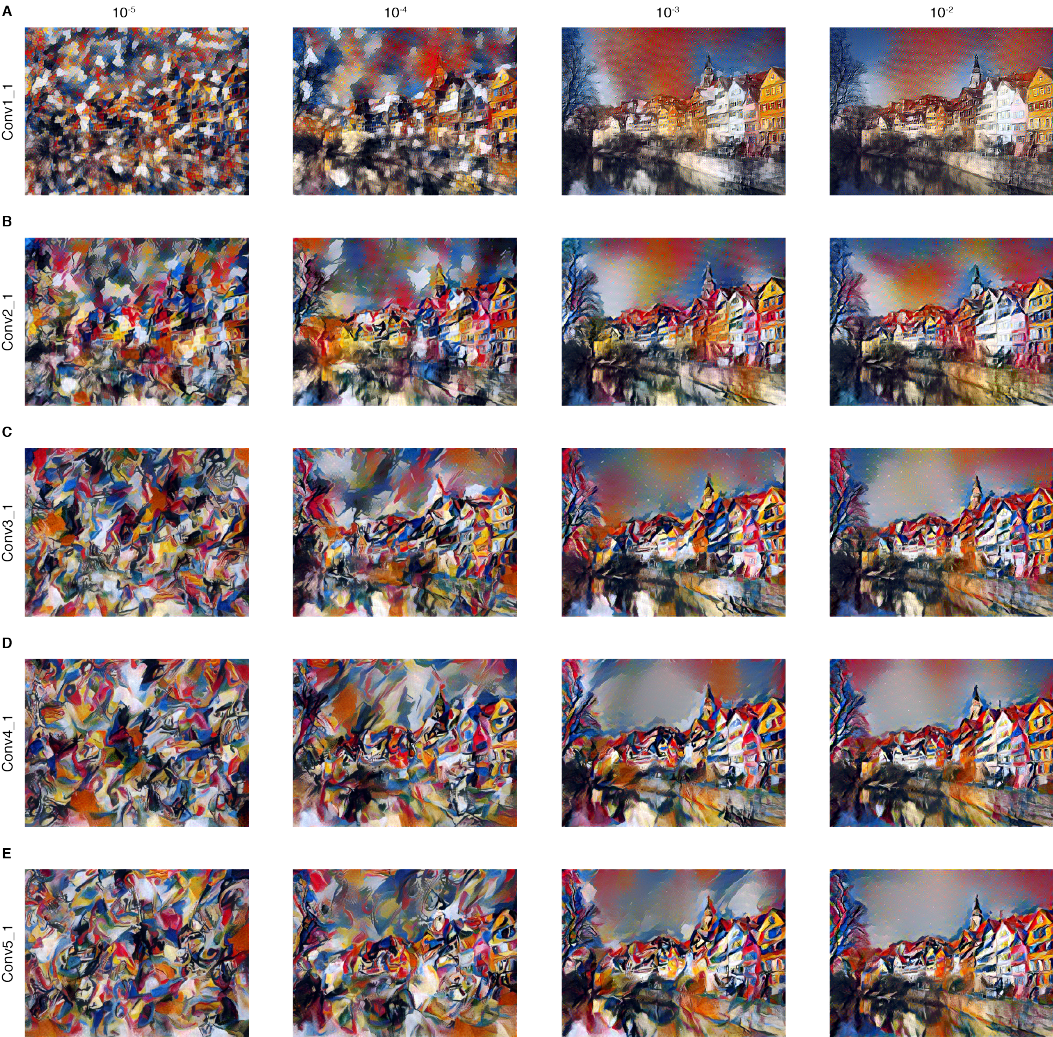
\includegraphics[width=0.6\textwidth]{figures/composition.png}
	\caption{Encoding with different weights in different layers \citep{Paper1}}
	\label{fig:Composition}
\end{figure*}
Here we see different relative weightings of $\alpha$ and $ \beta$ in the columns. The number above shows the ratio $\alpha/\beta$ . Clearly, if we have unbalanced weights, we either have to much of the original art image, so we can't really see the content anymore, or to much content, leaving the style of the picture very similar to the original photo. Also in the rows we can see the effect of choosing different layers for the computation. If we include higher levels, the output has bigger and more complex patches of "style". This could happen because of bigger style complexity in higher layers as can be seen in figure \ref{fig:NetworkModel}. With the right weights we now have a method to mix the content and the style from two different images. 
\section{Video recognition}
We now want to apply this method to a whole video sequence. If we just apply the the style of an artwork to every frame of the video independently the sequence gets very uncertain and shines unsteadily. This result was expected since the style transfer task is unstable and every image has multiple possible solutions that minimize the Loss-function. There are multiple methods to stabilize the video and also retain smooth transitions between the frames. 
\subsection{Short-term consistency}
Since every frame gets initialized with an independent white noise image we get different minima for every frame of the video sequence. To counter this the idea is to initialize the frame $i+1$ with the help of frame $i$. We initialize the optimization for the frame with the style of frame before. This means we still have to compute the style for the first frame randomly. But all the frames after that should be consistent with the style. Spaces which do not change in between frames remain with the appearance from before. Objects in motion however are still a problem. The objects get styled incorrectly. So to extend our approach we also calculate the optical flow of the frame and try to integrate it into our computation for the style. We now initialize the frame $i+1$ with the frame we stylized before, but also add in the optical flow between the two frames. As a formula: $$x'^{(i+1)} = w_i^{i+1}(x^{(i)})$$ $w_i^{i+1}$ is the estimated optical flow between the content images $p^{(i)}$ and $ p^{(i+1)}$. 
To estimate and generate the optical flow two different flow estimation algorithms were used, DeepFlow and EpicFlow \citep{Paper2}. 
\subsection{Temporal consistency}
Since the consistency between neighboring frames wasn't strong enough, we need a penalty to deviation between frames. This means we introduce an extra Loss function to make sure that the deviation between two adjacent frames is not too big. For the function we also use the optical flow. We estimate the forward flow and the backward flow and try to minimize the difference between the backward flow and the warped flow. As a loss function we get: $$\mathcal{L}_{temporal}(x,w,c) = \frac{1}{D} \sum_{k=1}^D c_k \cdot (x_k - w_k)^2$$ With $c \in [0,1]^D$ as a per-pixel weighting of the loss and $D$ as the dimensionality of the image. The weights are important for occluded areas where we cannot really estimate the optical flow. 
\subsection{Longterm consistency}
With our temporal consistency we still have trouble with occluded areas. Even though we ignore them in our Loss function, we still get styling errors here. The main complication is that when an are gets occluded and un-occluded, the area gets a completely new style. This happens because our algorithm does not remember the style of the area when it gets occluded. To tackle this problem we introduce an additional Loss function for the longterm consistency. Here we penalize deviations from frames from longer ago. We basically use the same Loss function as before, only we also look at frames from longer before. 
\subsection{Multi-pass algorithm}
At last we need to counter an effect of our previous stylizations. The output of the algorithm lacked contrast and was less diverse at the borders. To reverse this effect, a multi-pass algorithm was used. The sequence was processed in multiple passes and from different directions. This countered the information flow from the borders to the center. In every pass we start with an different random initialization and blend non-occluded areas of our frame with previous ones warped according to the optical flow. This in total led to a more diverse image. 
\section{Conclusion}
With help of the newly introduced Loss-functions to achieve short- and long-term consistency and a multi-pass algorithm to achieve a diverse and high-contrast video. This means production of stable and high-quality stylized videos is possible. Even occluded videos or films with fast motions can be handled. 





\bibliographystyle{ACM-Reference-Format}
\bibliography{lit.bib}


\end{document}
